% !TeX root = main.tex
%! Author = Matteo
%! Date = 10/06/2022

% Preamble
%\documentclass[11pt]{book}

\documentclass[12pt, letterpaper, openright, a4paper]{report}
% Packages
\usepackage{amsmath}
\usepackage[italian,english]{babel}
\usepackage{newlfont}
\usepackage{gensymb}
\usepackage{lipsum}
\usepackage{hyperref}
\usepackage{xr}
\usepackage{graphicx}
\usepackage{caption,subcaption}
\usepackage{amsfonts}
\usepackage{listings}
\usepackage{mathtools}
\usepackage{footmisc}
%Spacing del testo
\usepackage{setspace} 
\onehalfspacing




%Per tabelle
\usepackage{caption, tabularx, ragged2e, array}

%Per i plot
\usepackage{pgfplots}

%Gestione degli alberi delle strutture delle cartelle
\usepackage{forest}

\definecolor{folderbg}{RGB}{124,166,198}
\definecolor{folderborder}{RGB}{110,144,169}


\def\Size{4pt}
\tikzset{
      folder/.pic={
        \filldraw[draw=folderborder,top color=folderbg!50,bottom color=folderbg]
          (-1.05*\Size,0.2\Size+5pt) rectangle ++(.75*\Size,-0.2\Size-5pt);  
        \filldraw[draw=folderborder,top color=folderbg!50,bottom color=folderbg]
          (-1.15*\Size,-\Size) rectangle (1.15*\Size,\Size);
      }
    }

%Comando per fare reference ad altri file
\makeatletter
\newcommand*{\addFileDependency}[1]{% argument=file name and extension
  \typeout{(#1)}
  \@addtofilelist{#1}
  \IfFileExists{#1}{}{\typeout{No file #1.}}
}
\makeatother

\newcommand*{\myexternaldocument}[1]{%
    \externaldocument{#1}%
    \addFileDependency{#1.tex}%
    \addFileDependency{#1.aux}%
}

%Comando per scrivere c++
\newcommand{\CPP}{C\nolinebreak\hspace{-.05em}\raisebox{.4ex}{\tiny\bf +}\nolinebreak\hspace{-.10em}\raisebox{.4ex}{\tiny\bf +}}
\def\CPP{{C\nolinebreak[4]\hspace{-.05em}\raisebox{.4ex}{\tiny\bf ++}}}

%Comandi per scrivere parole in inglese
\newcommand{\ML}{\textit{Machine Learning}}
\newcommand{\DL}{\textit{Deep Learning}}
\newcommand{\DS}{\textit{Dataset}}
\newcommand{\ds}{\textit{dataset}}

%COmandi per accenti
\newcommand{\Eaccentata}{\'E}

%Comando per mettere le angle bracket e minore e maggiore
\newcommand{\<}{\textless}
%\newcommand{\>}{\textgreater}

\newcommand{\anglebra}[1]{\textlangle{#1}\textrangle}

%Comando per typesettare comandi
\newcommand{\command}[1]{\[\$ \; \textit{#1}\]}
\newcommand{\args}[1]{\textless #1\textgreater}

%Comando per typesettare codice

\newcounter{code}
\renewcommand{\lstlistingname}{Snippet}
\lstdefinestyle{verbo}{  % code typesetting optins
    basicstyle=\small\ttfamily,
    breaklines=true,
    numbers=left,
    breakatwhitespace=true,
    language=Python,
    tabsize=1,
    resetmargins=true,
    xleftmargin=0pt,
    frame=single,
    showstringspaces=false
}
\lstnewenvironment{code}[1][]
 {\lstset{style=verbo,#1}}
 {}

%Comandi per la generazione di grafi
\usepackage{tikz}
\usetikzlibrary{arrows}


%Comandi per i record di dati
\newcommand{\record}[1]{\anglebra{\textit{#1}}}

%Comando per argmax e min
\DeclareMathOperator*{\argmax}{arg\,max}
\DeclareMathOperator*{\argmin}{arg\,min}


%Comando per il referecing di capitoli
\NewDocumentCommand{\chapref}{s m}{Chapter~\ref{#2}\IfBooleanF{#1}{ \nameref{#2}}}

% Per il frontespizio
\textwidth=450pt\oddsidemargin=0pt\evensidemargin=0pt

% Per titolo capitoli
\usepackage{fancyhdr}
\pagestyle{fancy}
\renewcommand\chaptermark[1]{\markboth{\thechapter\ #1}{}}
\fancyhead[L]{\nouppercase{\leftmark}}
\fancyhead[R]{\thepage}

%Definizioni
\newtheorem{definition}{Definizione}

% Documents
\begin{document}
    \begin{titlepage}
\begin{center}
{{\Large{\textsc{Alma Mater Studiorum $\cdot$ Universit\`a di
Bologna}}}} \rule[0.1cm]{15.8cm}{0.1mm}
\rule[0.5cm]{15.8cm}{0.6mm}
{\small{\bf SCUOLA DI SCIENZE\\
Corso di Laurea Triennale in Informatica }}
\end{center}
\vspace{15mm}
\begin{center}
{\LARGE{\bf Tecniche di deep learning}}\\
\vspace{3mm}
{\LARGE{\bf per il riconoscimento}}\\
\vspace{3mm}
{\LARGE{\bf di errori nel codice}}\\
\end{center}
\vspace{40mm}
\par
\noindent
\begin{minipage}[t]{0.47\textwidth}
{\large{\bf Relatore:\\
Chiar.mo Prof.\\
Maurizio Gabbrielli}}
\end{minipage}
\hfill
\begin{minipage}[t]{0.47\textwidth}\raggedleft
{\large{\bf Presentata da:\\
Matteo Vannucchi}}
\end{minipage}
\vspace{20mm}
\begin{center}
{\large{\bf Sessione I\\%inserire il numero della sessione in cui ci si laurea
Anno Accademico 2021-2022}}%inserire l'anno accademico a cui si è iscritti
\end{center}
\end{titlepage}

    \makeatletter
\if@titlepage
  \newenvironment{abstract}{%
      \titlepage
      \null\vfil
      \@beginparpenalty\@lowpenalty
      \begin{center}%
        \bfseries Abstract
        \@endparpenalty\@M
      \end{center}}%
     {\par\vfil\null\endtitlepage}
\else
  \newenvironment{abstract}{%
      \if@twocolumn
        \section*{\abstractname}%
      \else
        \small
        \begin{center}%
          {\bfseries \abstractname\vspace{-.5em}\vspace{\z@}}%
        \end{center}%
        \quotation
      \fi}
      {\if@twocolumn\else\endquotation\fi}
\fi
\makeatother

\begin{abstract}
  Il ruolo dell'informatica, in un mondo in progressiva digitalizzazione di ogni singolo aspetto della vita dell'individuo, è ormai diventato chiave del suo funzionamento. 
  Con l'aumentare della complessità del codice e delle dimensioni dei progetti, il rilevamento di errori diventa sempre di più un'attività difficile e lunga. Meccanismi di analisi
  del codice sorgente tradizionali sono esistiti fin dalla nascita dell'informatica stessa, e il loro ruolo all'interno della catena produttiva di un team di programmatori non è mai stato cosi fondamentale come 
  lo è tuttora. Questi meccanismi di analisi però non sono esenti da problematiche: il tempo di esecuzione su progetti grandi e la percentuale di falsi positivi possono infatti diventare un grosso problema.
  Per questi motivi meccanismi fondati su \ML, e più in particolare \DL, sono stati sviluppati negli ultimi anni. Questo lavoro di tesi si pone quindi l'obbiettivo di esplorare e sviluppare un modello per il riconoscimento di errori
  in un qualsiasi file sorgente scritto in linguaggio sia C sia \CC.


\end{abstract}

    \tableofcontents
    \listoffigures
    \listoftables

    \chapter*{Introduzione}
    \chapter{Introduzione teorica}\label{chap:introduzione_teorica}

\section{Code2Vec}\label{sec:code2vec}

\subsection{Meccanismo di attenzione}

\subsection{AstContext}\label{subsec:astcontext}
    \chapter{Dataset}\label{chap:dataset}
In questo capitolo tratteremo la generazione del dataset posto alla base del modello che andremo a creare poi nel \autoref{chap:modello}. 
In prima istanza vedremo la versione originale utilizzata e poi come è stata migliorata tramite l'utilizzo di ulteriori analizzatori per aumentarne la precisione delle rilevazioni, riducendone il numero di falsi positivi.
In un secondo momento verrà esposto come le rilevazioni degli analizzatori statici sono utilizzate per la associazione tra un \textit{code snippet} e il relativo errore, infine come da quest'ultimo venga ricavato il codice in formato di \textit{ast context vector}.

\section{Dataset originale}
Come detto in precedenza questo dataset non è stato generato partendo da zero, ma facendo riferimento al dataset creato da \cite{gelman2019source}. Il dataset è composto da circa 3000 progetti di GitHub, scritti in linguaggi C e \CPP,
 che rispettano due requisiti: hanno una licenza ridistribuibile e hanno almeno 10 stelle.
 Il secondo requisito serve per garantire che i progetti all'interno del dataset soddisfino degli standard di qualità, infatti come precedenti studi hanno mostrato (come ad esempio \cite{papamichail2016user}) si può utilizzare il numero
 di stelle su GitHub come un \textit{proxy} per la qualità del codice stesso.

Il dataset contiene per ogni progetto una serie di analisi effettuate: l'analisi di Doxygen che estrae le coppie codice-commento e l'analisi di Infer \footnote{Infer è un analizzatore di codice statico} che produce un report di analisi statica degli errori.
L'analisi di Doxygen è stata scartata, in quanto non utile allo scopo di questo lavoro. In \autoref{fig:dir_struct} si può vedere la struttura tipica di uno dei circa 3000 progetti presenti.
Come si può notare, ogni directory contiene un Makefile necessario per l'esecuzione corretta di alcuni analizzatori.
\begin{figure}
    \centering
    \scalebox{0.6}{
        \begin{forest}
            for tree={
                font=\ttfamily,
                grow'=0,
                child anchor=west,
                parent anchor=south,
                anchor=west,
                calign=first,
                inner xsep=7pt,
                edge path={
                  \noexpand\path [draw, \forestoption{edge}]
                  (!u.south west) +(7.5pt,0) |- (.child anchor) pic {folder} \forestoption{edge label};
                },
                % style for your file node 
                file/.style={edge path={\noexpand\path [draw, \forestoption{edge}]
                  (!u.south west) +(7.5pt,0) |- (.child anchor) \forestoption{edge label};},
                  inner xsep=2pt,font=\small\ttfamily
                             },
                before typesetting nodes={
                  if n=1
                    {insert before={[,phantom]}}
                    {}
                },
                fit=band,
                before computing xy={l=15pt},
              }  
        [Project-name
          [source
            [Project-name
                [Makefile, file]
                [File1.c, file]
                [File2.c, file]
                [..., file]
                [Folder1]
                [Folder2]
                [...]
            ]
          ]
          [derivatives
            [
                Infer-out
                [bugs.txt, file]
            ]
            ]
            [LICENSE, file]
            [url, file]
        ]
        \end{forest}
    }
    %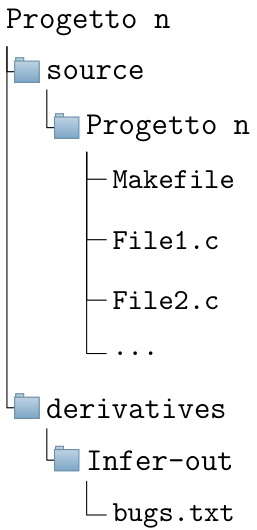
\includegraphics[scale=0.3]{images/immagineStrutturaDirectoryIniziale.png}
    \caption{La struttura della directory di un progetto del dataset iniziale}
    \label{fig:dir_struct}
\end{figure}


%Figura della struttura delle directory


%\subsection{Dataset originale}
 

%\subsection{Analizzatori utilizzati}

\section{Analizzatori di codice statici}
Un'analizzatore di codice è un programma che prende in input uno o più file e genera un report degli errori, cioè una lista di coppie del tipo $<$Errore, Posizione$>$, spesso in forma di file testuale. Di questi analizzatori ne esistono due macro categorie: statici e dinamici. 
Gli analizzatori statici sono programmi che effettuano controlli solo sul codice a livello testuale e che quindi non eseguono in nessuna maniera il codice. Gli analizzatori dinamici sono invece analizzatori più complessi che effettuano controlli a \textit{run-time},
andando quindi ad'eseguire il codice stesso.

Gli analizzatori non sono però perfetti, infatti nell'insieme degli errori trovati si possono spesso trovare dei falsi positivi: frammenti di codice segnalati come erronei che in realtà non presentano nessun tipo di problema.


\subsection{Analisi a livello di progetto} \label{subsec:compile_database}
La maggior parte degli analizzatori statici, inoltre, è in grado di lavorare a livello di progetti, andando a risolvere correttamente gli \textit{include} (nel caso di C e \CPP) e generando un output più significativo. 
Alcuni di questi, per far ciò, hanno bisogno di un file chiamato \textit{compilation database} che mantiene informazioni sulla compilazione dei file del progetto. 
Per soddisfare questo requisito esistono strumenti appositi che utilizzano il Makefile per generarlo, nel caso di questo lavoro è stato utilizzato un programma chiamato Bear.


\subsection{Analizzatori utilizzati}
Come analizzatori sono stati utilizzati i seguenti quattro:
%Come analizzatori statici ulteriori da aggiungere in più a Infer, di cui ogni elemento del dataset ha già l'analisi sua associata, sono stati scelti i seguenti tre:
    \begin{itemize}
        \item L'analizzatore Cppcheck che ha tra i suoi punti di forza il minimizzare il numero di falsi positivi.
        \item GCC che, oltre ad'essere un compilatore, ha anche funzionalità per l'analisi statica dei programmi attraverso il parametro \textit{-fanalyzer}.
        \item Il compilatore Clang, che attraverso un suo tool chiamato Clang-Check, è in grado di effettuare analisi statiche.
        \item L'analizzatore Infer il cui dataset è già dotato delle analasi.
    \end{itemize}
Non sono stati usati analizzatori dinamici, questo perché il loro utilizzo in modo automatizzato è un'operazione estremamente complicata e al di fuori della portata di questo lavoro;
infatti quasi tutti i programmi prendono dei parametri o degli input durante l'esecuzione, ma fornire questi dati in modo consistente, sensato per il programma e in modo automatizzato è praticamente impossibile.

L'utilizzo di essi potrebbe però portare a risultati molto interessanti poiché parte dei falsi positivi degli analizzatori statici deriva dal non poter decidere se frammenti di codice sono o non sono eseguiti e di conseguenza devono analizzarli tutti.
Può infatti succedere che l'analizzatore statico riferisca errori presenti in codice mai eseguito mentre, in questo caso, quello dinamico, correttamente, non lo riferirebbe.

\section{Utilizzo efficace di processori multicore}
L'ultimo argomento da discutere prima di illustrare i passaggi della generazione del dataset, è il tempo di esecuzione. 
Vista la mole di progetti e le loro dimensioni non irrilevanti, se eseguissimo in modo \textit{naive} la generazione del dataset, avremmo tempi di analisi che potrebbero estendersi a periodi di più giorni.
Dal momento che il processore a disposizione è \textit{multicore}, è stato deciso di ridurre i tempi di esecuzione delle fasi della generazione sfruttando appieno questa caratteristica.
Python attraverso la sua libreria \textit{multiprocessing} permette infatti di eseguire la computazione in processi diversi, andando a ridurre drasticamente il tempo delle operazioni.
Quindi tutte le operazioni di seguito descritte, anche non facendone più menzione, saranno eseguite in questa modalità.

\section{Prima fase: generazione dei report degli errori}
La prima fase della generazione del dataset consiste quindi nell'utilizzare i tre analizzatori scelti per generare ulteriori report degli errori, in particolare:
    \begin{itemize}
      \item Per eseguire l'analizzatore di GCC vengono prima raccolti tutti i file sorgenti del progetto, cioè tutti quei file con estensione '.c', '.cpp' o '.h'. Una volta fatto ciò viene eseguito il seguente comando:
            \command{gcc -fanalyzer -Wall \args{files} 2\textgreater  gcc-bugs.txt}

            Il prodotto di questo comando sarà un unico file contenente tutti gli errori e la loro posizione indicata con il percorso relativo del file e il numero sia della riga sia della colonna.
      \item Clang-check invece può essere eseguito su una cartella occupandosi lui di trovare i file da analizzare.
             Non viene però utilizzato in questa modalità per una motivazione principale: al posto di utilizzare il percorso assoluto o relativo di un file, clang-check utilizza solamente il nome di questo. Può succedere però che in grandi progetti si abbiano file chiamati uguali ma in cartelle diverse e quindi la loro distinzione sarebbe impossibile.
             Per risolvere questo problema viene eseguito individualmente su ogni file tramite il comando:
              \command{clang-check -{}-analyze -p compile\_commands.json \args{file}}
            Gli output generati dall'esecuzione di questi comandi vengono poi processati andando a sostituire i nomi dei file con il loro percorsi relativi, infine sono uniti tutti insieme. 
            Come si può notare viene utilizzato un file chiamato compile commands.json che è il file che è richiesto da certi analizzatori statici, come già detto nella \autoref{subsec:compile_database}.
      \item Per finire viene poi eseguito cppcheck che invece non ha bisogno di nessun aggiustamento e si può eseguire direttamente su tutta la cartella contenente i sorgenti con il seguente comando:
            \command{cppcheck \args{cartella\_sorgenti} -{}-output-file=cppcheck-bugs.txt}
    \end{itemize}
    In \autoref{fig:grafo_errori_generati} possiamo vedere quanti errori sono stati generati da ogni singolo analizzatore.


    \begin{figure}
      \centering
      \begin{tikzpicture}
      \begin{axis}[
      width  = \textwidth * 0.7,
      height = 7cm,
      major x tick style = transparent,
      ybar=0.1pt,
      bar width=30pt,
      ymajorgrids = true,
      ylabel style={yshift=2ex},
      xlabel style={yshift=-1ex},
      xlabel=Analizzatore,
      ylabel=Numero di errori generati,
      symbolic x coords={clang,gcc,cppcheck, infer},
      xtick = data,
      scaled y ticks = false,
      ymin=0,ymax=35000,
      ytick style={draw=none},
      %extra y ticks = 100,
      %extra y tick labels={},
      %extra y tick style={grid=major,major grid style={very thick,draw=red}}
      ]
      \addplot table {
        Analizzatore Numero
        clang 9855
        gcc 30386
        cppcheck 15230
        infer 29950
      };
      \end{axis}
      \end{tikzpicture}
      \caption{Numero di errori generati da ogni analizzatore}
      \label{fig:grafo_errori_generati}
  \end{figure}


\section{Seconda fase: aggregazione dei report degli errori}
Dopo la prima fase, descritta nella sezione precedente, avremo come risultato quattro report di errori per ogni progetto in file separati. Questi report si distinguono per due caratteristiche principali: la struttura del file e la nomenclatura degli errori. 
Per poter andare ad utilizzare questi risultati e fare quindi l'aggregazione di essi, dovremo effettuare due trasformazioni: un \textit{parsing} e una \textit{normalizzazione}.


\subsection{Parsing dei report}
Il \textit{parsing} è l'analisi di un dato in forma testuale per identificarne le sue componenti principali dove, in questo caso, sono la tipologia di errore e la sua posizione. 
Nel nostro caso è possibile eseguire il parsing tramite delle specifiche \textit{regex} che, avendo diversi formati di file, saranno diverse per ognuno degli analizzatori.
Il risultato del parsing sono quindi tanti record nella forma \record{errore, posizione}, dove la posizione indica sia il percorso del file sia la riga e la colonna dell'errore.

\subsection{Normalizzazione}
Per \textit{normalizzazione} si intende il processo di uniformare ad'un unico spazio di valori i dati forniti. Questo fase è fondamentale poiché i vari analizzatori forniscono lo stesso tipo di errore sotto nomi diversi. 
Per fare un esempio possiamo guardare la \autoref{tab:nomenclature} che riassume le diverse nomenclature per il tipo di errore 'memory leak'. 

\vskip1cm
    \noindent\setlength\tabcolsep{4pt}%
    \begin{tabularx}{\linewidth}{|l|c|*{4}{>{\RaggedRight\arraybackslash}X|}}
      \hline
      Forma normalizzata & Infer & Clang & Cppcheck & GCC \\ [0.5ex]
      \hline
      Memory leak  &  MEMORY\_LEAK  & unix.Malloc, ... & memleak, memleakOnRealloc, ... &  Wanalyzer-malloc-leak\\
      \hline
    \end{tabularx} 
    \captionof{table}{Tabella delle diverse nomenclature per l'errore 'memory leak'} \label{tab:nomenclature}
\vskip1cm

Notiamo inoltre un concetto fondamentale: analizzatori diversi producono analisi a granularità diverse. 
Si può osservare granularità maggiore, per il tipo di errore 'Memory leak', da parte di Cppcheck e Clang nella \autoref{tab:nomenclature}.
Infatti tutti e due definiscono più tipologie di errori che però, per convezione di questo progetto, vengono raggruppate in un'unica macro categoria.
Al contrario ci sono invece casi in cui un analizzatore non ha sensibilità sufficiente per distinguere fra due o più categorie di errori, in questa situazione un errore di quel tipo viene normalizzato in un errore per ogni categoria che potrebbe rappresentare, si può vedere ciò nella \autoref{tab:granularità}.
Nella eventualità quindi che Clang riferisca un errore di tipo 'unix.Malloc', dopo la fase di normalizzazione avremo due errori nella stessa posizione: uno di tipo 'Memory leak' e uno di tipo 'Use after free'. 

\begin{center}
  \begin{tabular}{|c|c|}
    \hline
    Forma normalizzata & Clang  \\
    \hline
    Memory leak  &  unix.Malloc, ... \\
    \hline
    Use after free & unix.Malloc, ... \\
    \hline
  \end{tabular}
  \captionof{table}{Tabella che mostra come un determinato errore di un analizzatore potrebbe corrispondere a più forme normalizzate} \label{tab:granularità}
\end{center} 

Per effettuare la normalizzazione è stata quindi sviluppata una tabella che associa ad ogni forma normalizzata degli errori le forme definite dagli analizzatori usati.
Questa tabella è stata poi utilizzata come dizionario per convertire le tipologie di errori.


%vengono definiti più errori, nella stessa posizione, per ogni categoria che potrebbe rappresentare quell'errore.

\subsection{Aggregazione dei report}
Una volta definite le trasformazioni da effettuare possiamo introdurre l'effettivo argomento di questa sezione, cioè l'aggregazione dei quattro file prodotti dagli analizzatori.
Il processo di aggregazione permette di generare un unico report finale degli errori, andando a selezionare soltanto gli errori che sono stati individuati da almeno $n$ analizzatori. 
Modificando il parametro $n$ andremo, di conseguenza, a modificare la precisione e la dimensione del dataset nel seguente modo:
  \begin{itemize}
    \item Ponendo $n=1$ avremo la dimensione massima del dataset, in cui ogni singolo errore riportato viene mantenuto, a scapito però di un numero di falsi positivi più grande.
          Notiamo comunque, e questo vale per tutti i valori di $n$, che nel caso di errori duplicati ne viene sempre inserito solo uno.
    \item Ponendo $n=2$ avremo un bilanciamento fra precisione e dimensione del dataset. Vengono infatti selezionati tutti gli errori riferiti da almeno due analizzatori. 
        %Infatti come è stato notato empiricamente è alquanto raro che più di due degli analizzatori individuino un specifico errore,
          %quindi con $n=2$ manterremo comunque un sufficiente numero di dati migliorandone però la precisione.
    \item Ponendo $n>2$ invece il numero di errori selezionato diventa così basso che renderebbe difficile addestrare il modello, il numero di falsi positivi però diminuisce di conseguenza.
  \end{itemize}
Si può vedere in modo più chiaro come al variare del valore di $n$ cambi il numero di errori ottenuti in \autoref{fig:grafo_aggregazione}.
Nel caso di questo lavoro sono stati utilizzati dataset sia derivanti dal porre $n=1$ sia dal porre $n=2$.

\begin{figure}[h]
    \centering
    \begin{tikzpicture}
    \begin{axis}[
    width  = \textwidth * 0.7,
    height = 7cm,
    major x tick style = transparent,
    ybar=0.1pt,
    bar width=30pt,
    ymajorgrids = true,
    ylabel style={yshift=2ex},
    xlabel=Numero di occorrenze minimo ($n$),
    ylabel=Numero di errori ottenuti,
    xtick = data,
    scaled y ticks = false,
    ymin=0,ymax=50000,
    ytick style={draw=none},
    %extra y ticks = 100,
    %extra y tick labels={},
    %extra y tick style={grid=major,major grid style={very thick,draw=red}}
    ]
    \addplot table {
      N Numero 
      1 45606
      2 5423
      3 1049
      4 433
    };
    \end{axis}
    \end{tikzpicture}
    \caption{Numero di errori aggregati ottenuti in variazione del numero $n$ di occorrenze minime}
    \label{fig:grafo_aggregazione}
\end{figure}

\section{Terza fase: associazione tra errore e codice}
Lo scopo di questa fase è quello di mappare la posizione di ogni singolo errore ad un determinato \textit{code snippet}. 
Prima di far ciò va definito però a che livello eseguire le analisi e quindi le successive predizioni del modello.
Le possibili strade che si possono intraprendere sono:
  \begin{itemize}
    \item A livello di file. Facendo ciò, dato un errore, il \textit{code snippet} che associamo è il codice sorgente del intero file. 
          Questo metodo ha due vantaggi principali: la semplicità e la quantità d'informazioni codificate. 
          Ha però anche una serie di svantaggi: per il modello potrebbe essere troppo dispersivo per file grandi e, dal momento che un singolo file è probabile che contenga più errori, il modello dovrebbe restituire sequenze di predizioni.
    \item A livello di funzione. In questo caso si associa all'errore il blocco della funzione che lo racchiude.
          Il beneficio di ciò è la riduzione drastica del frammento di codice, rendendo più chiare le relazioni tra i vari elementi del codice e il tipo di errore.
    \item A livello di riga, in cui ad un dato errore associamo come code snippet solo la riga stessa. In questo caso la dispersione sarà minima ma allo stesso tempo lo sarà la quantità d'informazioni a disposizione.
  \end{itemize}

In \autoref{fig:trade_off} possiamo notare il \textit{trade-off} che avviene tra l'aumento della dimensione del code snippet e la quantità d'informazioni da esso incapsulata. 

\begin{figure}[h]
  \centering
  \begin{tikzpicture}
    \begin{axis}[
        xlabel={Quantita di informazioni},
        ylabel={Dispersività},
        yticklabels={,,},
        xticklabels={,,},
        xmin=0,    xmax=2, % Prima era 1 
        ymin=0,    ymax=1.718,
        axis line style={->},
        legend pos=south east
    ]
        \addplot[color=blue,domain=0:2,smooth, samples=400]{exp(x)-1};
        \addplot +[mark=none, color=red, dashed] coordinates {(0.5,0) (0.5, 0.649)};
        \addplot +[mark=none, color=red, dashed] coordinates {(0,0.649) (0.5, 0.649)};
    \end{axis}
    %
  \end{tikzpicture}
  \caption{\textit{Trade-off} che avviene tra la dispersività e la quantità di informazioni. Selezionando tanto codice avremo molte informazioni codificate ma aumenterà, allo stesso tempo, la dispersività, mentre selezionandone poco avremo poca dispersività ma potremmo perdere informazioni chiave.
    Le due linee rosse indicano un punto di bilanciamento tra i due.
  }
  \label{fig:trade_off}
\end{figure}

Nel lavoro svolto è stato scelto di eseguire le analisi a livello di funzione, andando però ad aumentare il quantitativo d'informazioni a disposizione aggiungendo un contesto della funzione (la cui definizione verrà data in seguito nella \autoref{subsec:context}). 
Facendo questa scelta, è possibile approssimare il problema ipotizzando che in una data funzione ci sia massimo un solo errore, rendendo quindi l'architettura del modello finale più semplice.

Una volta determinato il livello a cui svolgere le analisi possiamo tornare al problema principale: estrarre il codice della funzione che racchiude l'errore. 
Nonostante questo possa sembrare un problema semplice di analisi testuale vedremo come, in realtà, non lo sia.
Questo vale ancora di più per linguaggi come C e \CPP{} che, tramite la loro sintassi molto libera, rendono il tutto più complicato.
A supporto di ciò vediamo lo \autoref{code:esempio_codice_complesso}.

\begin{code}[language=c++, caption={Esempio di codice valido con struttura particolare}, label={code:esempio_codice_complesso}]
  #DEFINE OPENBRACKET {
  #DEFINE CLOSEBRACKET }
  void foo()OPENBRACKET
    int error = 5 / 0; // Linea contente l'errore

    /* Questo commento rende difficile l'individuazione del corpo della funzione }
    */

  CLOSEBRACKET
\end{code}
In questo frammento si possono individuare due fattori problematici: la presenza di parentesi graffe in commenti e l'utilizzo particolare di direttive define.
Se volessimo ricavare il corpo della funzione analizzando semplicemente il testo dovremmo trovare le parantesi graffe di apertura e chiusura di esso, ma i due fattori appena elencati e ulteriori non discussi rendono necessarie delle accortezze maggiori. 

Per risolvere questo problema utilizzeremo gli alberi di sintassi astratta.

\subsection{Generazione e parsing degli alberi di sintassi astratta}
Come accennato nella precedente sezione, in questo lavoro vengono utilizzati gli \textit{ast} come metodo per estrarre i blocchi delle funzioni e il loro relativo contesto.
Prima di tutto bisogna essere in grado di generare un albero di sintassi astratta dato un file sorgente.
Per far ciò viene utilizzato il compilatore Clang che, attraverso flag specifiche, è in grado di generare un albero rappresentato in formato JSON.
Più in particolare per ogni file sorgente che vogliamo analizzare viene eseguito il seguente comando:
  \command{
    clang -Xclang -ast-dump=json \args{file}
  }
Il risultato di questa operazione è un file in formato JSON che rappresenta la struttura dell'albero.
Prima però di proseguire, questo file viene caricato e trasformato in una struttura ad albero vera e propria.

Oltre alla struttura sintattica del codice, all'interno dei dizionari JSON, sono presenti informazioni ulteriori: indicazioni sulla posizione degli elementi, sui tipi, sui riferimenti esterni e molto altro.
Tutte queste informazioni vengono poi usate sia per estrarre il codice sia per estrarre il contesto della funzione. 

\subsection{Contesto di una funzione} \label{subsec:context}
Definiamo in fine cosa si intende con contesto di una funzione.
Il contesto di una funzione è l'insieme di tutti quei riferimenti esterni che vengono effettuati all'interno del corpo della funzione, possono includere:
  \begin{itemize}
    \item Funzioni esterne.
    \item Variabili esterne.
    \item Definizioni di tipo esterne. Visto che le definizioni di tipo possono dipendere da altri tipi non primitivi, in questo caso oltre al riferimento stesso vengono aggiunte anche le dipendenze di esso, dove per dipendenza di un tipo $t$ al tipo $v$ si intende che la dichiarazione di $t$ include il tipo $v$ (un esempio di ciò lo si può vedere nello \autoref{code:esempio_codice_grafo_dipendenze}).
  \end{itemize}
L'idea posta alla base dell'includere questo contesto nel risultato finale è il poter dare al modello il maggior numero d'informazioni possibili mantenendo comunque limitata la dimensione dello snippet.
Senza di questo, infatti, anche un umano potrebbe non essere in grado di comprendere il codice o non poterne trarre conclusioni significative su di esso. 
Guardando infatti lo \autoref{code:esempio_codice_grafo_dipendenze}, senza l'inclusione nel risultato finale della variabile globale non potremmo determinare che nella funzione \textit{foo} ci sia effettivamente un errore di divisione per zero.

\begin{code}[language=c++, caption={Esempio di codice con riferimenti esterni}, label={code:esempio_codice_grafo_dipendenze}]

  typedef int typeA;
  typedef typeA typeB; 

  typedef float typeC;

  int variabileGlobale = 0;

  int bar(){
    ...
  }

  void foo(){
    typeB variable = 1; //riferimento di tipo esterno
    int var = 5 / variabileGlobale // errore
    
    result = bar();
    ...
  }

\end{code}

\subsubsection{Estrazione del contesto}\label{sec:estrazione_contesto}
Per l'estrazione del contesto vengono utilizzate le informazioni codificate nell'albero di sintassi astratta prodotto da Clang.
Solamente per le definizioni di tipo vengono incluse anche le relative dipendenze e per far ciò viene costruito un grafo delle dipendenze.

Il grafo delle dipendenze è un grafo diretto in cui un vertice $v$ rappresenta una dichiarazione di tipo, mentre un arco $(u,v)$ rappresenta la dipendenza del tipo $u$ dal tipo $v$.
Prendiamo come esempio lo \autoref{code:esempio_codice_grafo_dipendenze}. 
Il contesto della funzione \textit{foo} in questo caso dovrà mantenere informazioni sulla definizione di \textit{typeB}, dipendente però dalla definizione del \textit{typeA}.
Bisogna quindi costruire il grafo delle dipendenze dei tipi utilizzando le informazioni contenute all'interno dell'albero di sintassi astratta.
Possiamo vedere quindi il grafo delle dipendenze per questo specifico frammento di codice in \autoref{fig:grafo_dipendenze}.


\begin{figure}[h]
  \centering
  \begin{tikzpicture}
    \tikzset{vertex/.style = {shape=circle,draw,minimum size=1.5em}}
    \tikzset{edge/.style = {->,> = latex'}}
  
    % vertices
  \node[vertex] (typeB) at  (0,0) {typeB};
  \node[vertex] (typeA) at  (4,0) {typeA};
  \node[vertex] (int) at  (8,0) {int};
  \node[vertex] (typeC) at (2, -2) {typeC};
  \node[vertex] (float) at (6, -2) {float};
  %edges
  \draw[edge] (typeB) to (typeA);
  \draw[edge] (typeA) to (int);
  \draw[edge] (typeC) to (float);
  \end{tikzpicture}
  \caption{Grafo delle dipendenze di tipo per lo \autoref{code:esempio_codice_grafo_dipendenze}}
  \label{fig:grafo_dipendenze}
\end{figure}

Per poter ricavare le dipendenze delle dichiarazioni di tipo, una volta costruito il grafo, si può eseguire una visita in ampiezza partendo dal riferimento esterno stesso.
Nel caso della funzione \textit{foo} otterremo quindi, visto il riferimento esterno al tipo \textit{typeB}, due definizioni di tipo, quelle di \textit{typeB} e \textit{typeA}.  

\subsection{Esempio di risultato finale}
Riprendendo sempre lo \autoref{code:esempio_codice_grafo_dipendenze} avremo che il risultato finale dell'estrazione del metodo \textit{foo} è il seguente:


\begin{code}[language=c++, caption={Esempio di estrazione del codice della funzione foo insieme al contesto}, label={code:esempio_finale}]

  typedef int typeA;
  typedef typeA typeB; 
  int variabileGlobale = 0;
  int bar();
  void foo(){
    typeB variable = 1; //riferimento di tipo esterno
    int var = 5 / variabileGlobale // errore
    ...
  }

\end{code}

Notiamo quindi che la definizione del tipo \textit{typeC} non è inclusa poiché non utilizzata all'interno del corpo della funzione, mentre, sia la variabile globale, sia le due definizioni di tipo e sia la signature della funzione \textit{bar} sono incluse nel contesto.


\section{Quarta fase: Generazione degli AST-context}
Come accennato nell'introduzione teorica nel \autoref{chap:introduzione_teorica}, il modello che verrà utilizzato prenderà in input il codice sorgente processato sotto forma di vettore di \textit{ast contexts}, cioè delle triple della forma:
  \[\anglebra{x_s, p, x_t}\]

dove $x_s$ e $x_t$ sono rispettivamente il \textit{token start} e \textit{token end}, mentre $p$ è il \textit{path} come descritto in \cite{alon2019code2vec}.
A differenza però di come viene illustrato nell'articolo, in cui $x_s$ e $x_t$ sono un singolo valore, verranno utilizzati dei vettori di token di inizio e fine, nel tentativo di ridurre la dimensione dei vocabolari.
Per generare queste triple verrà utilizzato un tool chiamato \textit{Astminer}.

\subsection{AstMiner}
Astminer rappresenta il lavoro descritto in \cite{kovalenko2019pathminer} ed è un tool che permette di estrarre gli ast context da file sorgenti scritti in vari linguaggi come Python, C/\CPP{} e Java.
Può essere utilizzato in due modi differenti:
  \begin{itemize}
    \item Come una libreria di Kotlin/Java.
    \item Come un tool standalone della CLI. Questo sarà il modo che verrà utilizzato nel progetto essendo stato scritto tutto in Python.
  \end{itemize}
Lo strumento è configurabile in svariati modi; le uniche configurazioni rilevanti utilizzate sono:
  \begin{itemize}
    \item \'E stato utilizzato in modalità code2vec.
    \item Sono stati utilizzati i seguenti valori:
      \begin{itemize}
        \item maxPathContextsPerEntity $=200$. Questo valore rappresenta il numero massimo di \textit{ast context} da associare ad'un frammento di codice.
        \item maxPathLength $=20$. Questo valore rappresenta, invece, la lunghezza massima dei cammini.
        \item nodesToNumbers $=$ false. Infatti i vocabolari per la traduzione dei token verranno gestiti, non da Astminer, ma a livello dell'applicazione.
      \end{itemize}
  \end{itemize}
Come però già accennato nell'introduzione di questa sezione, il prodotto di Astminer in realtà non è esattamente uguale a quello illustrato nell'articolo di code2vec: invece che avere dei singoli valori per $x_s$ e $x_t$, Astminer produce in output \textit{ast context} che hanno token d'inizio e fine che sono vettori, scomponendo token complessi in token multipli.
\'E stato deciso di non modificare questa scelta poiché potrebbe portare ad una riduzione notevole della dimensione del vocabolario dei token, rendendo più significativo ogni singolo token.


\subsection{Generazioni vocabolari per i token e per i path}\label{subsec:vocab}
L'output dell'esecuzione di astminer, visto il parametro nodesToNumbers $=$ false, sono degli \textit{ast context} dove ogni token è ancora in formato letterale.
Per essere utilizzabile questo formato deve però prima essere trasformato in un valore intero.
Tale valore rappresenterà l'indice del token letterale all'interno di uno specifico vocabolario.

Più in particolare vengono creati due dizionari diversi:
  \begin{itemize}
    \item Un dizionario dei token degli elementi dei cammini ($p$) che d'ora in avanti chiameremo \textit{path vocab}.
    \item Un dizionario dei token degli elementi terminali (i valori $x_s$ e $x_t$ del \textit{ast context}). In questo caso lo chiameremo \textit{token vocab}.
  \end{itemize}
In \autoref{fig:grafo_vocab_size} possiamo vedere la dimensione dei due vocabolari.
Si può vedere come i due abbiano ordini di grandezza completamente differenti, questo può essere spiegato dal fatto che i token terminali racchiudono svariate tipologie di elementi come nomi di variabili e di metodi,
mentre i token dei cammini racchiudono solamente elementi sintattici fissi: costrutti come dichiarazioni, blocchi e operazioni.

  \begin{figure}
    \centering
    \begin{tikzpicture}
    \begin{axis}[
    width  = \textwidth * 0.7,
    height = 7cm,
    major x tick style = transparent,
    ybar=0.1pt,
    bar width=30pt,
    ymajorgrids = true,
    ylabel style={yshift=2ex},
    xlabel style={yshift=-1ex},
    xlabel=Vocabolario,
    ylabel=Numero di entry,
    symbolic x coords={token, path},
    xtick = data,
    scaled y ticks = false,
    ymin=0,ymax=50000,
    ytick style={draw=none},
    %extra y ticks = 100,
    %extra y tick labels={},
    %extra y tick style={grid=major,major grid style={very thick,draw=red}}
    ]
    \addplot table {
      vocab Numero
      token 45000
      path 50
    };

    \end{axis}
    \end{tikzpicture}
    \caption{Dimensione dei vocabolari dei token}
    \label{fig:grafo_vocab_size}
\end{figure}

\section{Risultato finale della generazione}
Il risultato dell'esecuzione di tutte le fasi menzionate è quindi un dataset formato da due elementi chiave:
    \begin{itemize}
        \item I \textit{code snippet} sotto forma di vettori di \textit{ast contexts} a cui vengono associate due informazioni:
        \begin{itemize}
            \item Un'etichetta indicante la tipologia di errore o la classificazione di una funzione senza errori.
            \item Il numero della riga dell'errore.
        \end{itemize}
        \item I due vocabolari dei token dei cammini e dei valori terminali.
    \end{itemize}
In \autoref{tab:tabella_errori} possiamo vedere riassunti sia le tipologie di errori estratti sia la loro frequenza.
    \begin{center}
      \begin{tabular}{|c|c|}
        \hline
        Errore & Osservazioni \\
        \hline
        No Error & 41417 \\
        \hline
        Memory leak & 1032 \\
        \hline
        Null dereference & 911 \\
        \hline
        Dead store & 791 \\
        \hline
        Variable not initialized & 325 \\
        \hline
        Resource leak & 122 \\
        \hline
        Double free & 83 \\
        \hline
        Pointer conversion & 80 \\
        \hline
        Data not initialized & 56 \\
        \hline
        Null argument & 31 \\
        \hline
        Use after lifetime & 16 \\
        \hline
        Division by zero & 10 \\
        \hline
        Integer overflow & 4 \\
        \hline
        Call and message & 3 \\
        \hline
        Array not initialized & 2 \\
        \hline
        Use closed file & 1 \\
        \hline
      \end{tabular}
      \caption{Tabella riassuntiva degli errori estratti con la loro frequenza}
      \label{tab:tabella_errori}
    \end{center}


\subsection{Estrazione di frammenti di codice senza errori}
Non è ancora stato menzionato come vengono ricavati i \textit{code snippet} che non presentano errori.
Il modello finale, infatti, dovrà essere in grado di determinare sia la tipologia di errore sia se effettivamente il frammento presenta errori.
Questa estrazione avviene in modo molto semplice: tutte le funzioni che non presentano errori sono estratte. 

Come però vedremo nel \autoref{chap:modello}, il dataset è molto sbilanciato verso la classe di non errore.
Per ridurre ciò, e anche per rendere il file del dataset più maneggiabile, vengono solo analizzati file che presentano errori.
Di conseguenza avremo che il numero di funzioni senza errori viene ridotto drasticamente. 

%\subsection{Fase 1: utilizzo di analizzatori statici per la generazione di report di errori}

%\subsection{Fase 2: aggregazione dei report}

%\subsbusection{Conversione degli errori}

%\subsection{Fase 3: }

%\subsection{Fase 4: generazione degli Ast Context}

%\section{Statistiche finali del dataset}
    \chapter{Il modello predittivo}\label{chap:modello}
Nel seguente capitolo affronteremo lo sviluppo del modello predittivo. 
Vedremo, prima di tutto, la struttura del modello discutendone i principali componenti e varie iterazioni di essa.  
In un secondo momento vedremo un problema fondamentale dato dalla distribuzione del dataset: il problema dello sbilanciamento.
Verrà anche introdotto brevemente come viene addestrato e le metriche utilizzato per valutarlo.
Infine saranno discussi i risultati ottenuti. 

\section{Struttura}
Come già introdotto nel \autoref{chap:introduzione_teorica}, questo modello si basa su un meccanismo di codifica del codice separato in due fasi:
    \begin{itemize}
        \item La prima codifica del \textit{code snippet} in un vettore di \textit{ast contexts}, effettuata a tempo di creazione del dataset, come già discusso nel \autoref{chap:dataset}.
        \item La seconda codifica del vettore di \textit{ast contexts} in un vettore di \textit{feature} attraverso meccanismi di \DL.
    \end{itemize}
Una volta ottenuto il vettore delle feature, vengono utilizzati due 'sotto reti' per la classificazione e la regressione. 
Possiamo vedere riassunta a grandi linee la struttura della rete in \autoref{fig:struttura}.

\begin{figure}[h]
    \centering
    \scalebox{0.8}{
        \begin{tikzpicture}[block/.style={draw, rectangle, minimum height=1cm}]
            \tikzset{vertex/.style = {shape=circle,draw,minimum size=1.5em}}
            \tikzset{edge/.style = {->,> = latex'}}
            
            \node[block] (input) at (0,0) {input};
            \node[block] (code2vec) at (4,0) {code2vec};

            \node[block] (classificazione) at (8, 2) {classificazione};
            \node[block] (regressione) at (8, -2) {regressione};
            
            \draw [edge] (input) to (code2vec);
            \draw [edge] (code2vec) to (classificazione);
            \draw [edge] (code2vec) to (regressione);
            
            \end{tikzpicture}
        }
      \caption{Struttura astratta del modello utilizzato}
      \label{fig:struttura}
\end{figure}


\begin{figure}[h]
    \centering
    \scalebox{0.8}{
        \begin{tikzpicture}[block/.style={draw, rectangle, minimum height=1cm}]
            \tikzset{vertex/.style = {shape=circle,draw,minimum size=1.5em}}
            \tikzset{edge/.style = {->,> = latex'}}

            \node[vertex] (xs0) at (0,3) {$x_s^0$};
            \node[vertex] (p0) at (0,1) {$p^0$};   
            \node[vertex] (xt0) at (0,-1) {$x_t^0$};
            
            \node at (1,3) {...};
            \node at (1,1) {...};
            \node at (1,-1) {...};


            \node[vertex] (xsc) at (2,3) {$x_s^c$};
            \node[vertex] (pc) at (2,1) {$p^c$};   
            \node[vertex] (xtc) at (2,-1) {$x_t^c$};


            \node[vertex] (mask) at (1,-3) {$m$};


            \node[vertex] (xs) at (4,3) {$x_s$};
            \node[vertex] (p) at (4,1) {$p$};   
            \node[vertex] (xt) at (4,-1) {$x_t$};



            \node[block] (classificazione) at (15, 2) {classificazione};
            \node[block] (regressione) at (15, -2) {regressione};

            \node (input) at(3.5,0) {};

            \node[rectangle, draw,dotted,red, ultra thick,label={[red]code2vec}, minimum width=6cm,
            minimum height = 2cm] at(8,0) (code2vec) {};

            \draw  [decorate,decoration={brace,amplitude=10pt}] (2.75,3.5) -- (2.75,-1.5) node (vec) [black,midway,xshift=0.4cm, yshift=1.8cm, label={[rotate=-90]right:contexts vector}] {};
            
            \node [fit=(xs0) (p0) (xt0) (mask) (xsc) (pc) (xtc),draw,dotted,blue, thick,label={[blue]input}] {};
            %\node [fit=(code2vec) (vector),draw,dotted,red, ultra thick,label={[red]code2vec}] (code2vec) {};
            \node [fit=(classificazione) (regressione),draw,dotted,orange, ultra thick,label={[orange]predizione}] {};
        
            \draw[edge] (code2vec) to (classificazione);
            \draw[edge] (code2vec) to (regressione);

            \draw[edge] (input) to (code2vec);
            \end{tikzpicture}
        }
      \caption{Struttura del modello utilizzato}
      \label{fig:struttura}
\end{figure}


Nelle successive sezione, in maniera approfondita, le seguenti tematiche:
    \begin{itemize}
        \item La struttura degli input e come sono stati gestiti i cambiamenti della loro forma discussi in precedenza nel \autoref{chap:dataset}.
        \item La struttura del modello di classificazione.
        \item La struttura del modello di regressione.
    \end{itemize}


\subsection{Struttura degli input}
Il dataset generato nel \autoref{chap:dataset} contiene per ogni suo elemento un vettore di \textit{ast contexts}, cioè un vettore di triple della forma:
    \[(x_s, p, x_t)\]
tali per cui vale la seguente relazione:
    \[x_s, x_t \in \mathbb{N}^{l} \quad p \in \mathbb{N}^{k}\]
dove $l$ e $k$ rappresentano rispettivamente la lunghezza massima del vettore dei token di inizio/fine e la lunghezza massima del vettore dei cammini, fissate al momento della creazione del dataset (nel nostro caso $l=10$ e $k=20$).
Per poter essere inserito all'interno di un modello dobbiamo 























Come si può vedere nella \autoref{fig:struttura} l'input è formato da quattro vettori diversi:
    \begin{itemize}
        \item La tripla $(x_s, p, x_t)$ che rappresenta l'\textit{ast context}, tale per cui:
            \[x_s, x_t \in \mathbb{N}^{c \times l}, \quad p \in \mathbb{N}^{c \times k}\]
        dove $l$ e $k$ rappresentano rispettivamente la lunghezza massima del vettore dei token di inizio/fine e la lunghezza massima del vettore dei cammini (fissate al momento della creazione del dataset).
        , mentre $c$ rappresenta il numero di massimo \textit{ast context} per ogni dato del dataset.
        Succede spesso che i vettori non siano di lunghezza sufficiente, in questi casi vengono aggiunti degli elementi di \textit{padding}
        tali da raggiungere la lunghezza di $l$ o $k$. Questi elementi di \textit{padding} sono rappresentati da un valore particolare nei rispettivi vocabolari.
        \item Una vettore maschera $m$ di lunghezza $k$ definito nel seguente modo:
        \begin{align*}
                m_i =
                \begin{cases*}
                  1 & se $p_i$ non è padding \\
                  0 & altrimenti
                \end{cases*}
        \end{align*}
        Non è invece definito un vettore maschera per i vettori dei token d'inizio e fine, questo perché l'implementazione avrebbe aumentato di troppo la dimensione della rete.
    \end{itemize}
Come già accennato 
\subsection{Classificazione}
L'obbiettivo della classificazione in questo modello è il predire la classe di errore o l'assenza di errore. 
Il modello, di conseguenza, in output dovrà fornire un vettore $c$ tale per cui per ogni $i$:
\[0 < c_i < 1\]
avremo quindi che il vettore $c$ è una \textit{distribuzione di probabilità} delle classi da predire.
Di conseguenza la classe con maggior probabilità sarà la classe predetta. Più formalmente la classe predetta $i$ sarà:
    \[\argmax_i c_i\]
Nel lavoro svolto la rete di classificazione è costituita da una serie di \textit{hidden dense layer} culminanti in un \textit{layer} di predizione che utilizza come funzione di attivazione la funzione \textit{softmax}.




\subsection{Predizione di regressione}


\subsection{Reshape degli input}

\subsection{Ulteriori architetture del modello provate}


\section{Soluzioni allo sbilanciamento del dataset}
    \subsection{Oversampling}
    \subsection{Loss pesata}
\section{Training}
\subsection{Metriche utilizzate}

\section{Risultati}
\subsection{Risultati dati dal test dataset}
\subsection{Risultati dati su codice creato al momento}
    \chapter{Conclusioni}

\section{Possibili migliorie}

    \cleardoublepage
    \bibliographystyle{plain}
    \addcontentsline{toc}{chapter}{\bibname}
    \bibliography{main}
\end{document}
